\documentclass[12pt,openright,oneside,a4paper,english,brazil]{abntex2}

\usepackage[T1]{fontenc}
\usepackage[utf8]{inputenc}
\usepackage{lmodern}
\usepackage{microtype}
\usepackage{booktabs}
\usepackage{tabularx}
\usepackage{array}
\usepackage{enumitem}
\usepackage{csquotes}
\usepackage{xurl}
\usepackage{tikz}
\usetikzlibrary{arrows.meta}
\usepackage{hyperref}
\usepackage[alf]{abntex2cite}

\hypersetup{hidelinks}
\setlist{nosep}
\newcolumntype{L}{>{\raggedright\arraybackslash}X}
\newcolumntype{P}[1]{>{\raggedright\arraybackslash}p{#1}}

\titulo{HIJACK: carrinho hackeável para o ensino de segurança em sistemas ciberfísicos}
\autor{Pedro Nascimento de Paiva Fernandes Neto \\ Carlos Roberto de Miranda Gomes Neto \\ Élisson Rian Félix Simas \\ Gustavo Henrique Assunção Paiva \\ Marcelo Jorge Oliveira de Albuquerque Melo \\ Matheus Felipe Duarte Dionísio \\ João Gonçalves de Souza Neto}
\local{Natal}
\data{2026}
\instituicao{Universidade Federal do Rio Grande do Norte}
\tipotrabalho{Relatório técnico}
\orientador[Professor:]{Alexandre Magnus Fernandes Guimarães}
\preambulo{Relatório final apresentado à disciplina Fundamentos de Circuito e Sistemas Controlados da Universidade Federal do Rio Grande do Norte.}

\renewcommand{\imprimircapa}{%
  \begin{capa}%
    \center
    {\ABNTEXchapterfont\large UNIVERSIDADE FEDERAL DO RIO GRANDE DO NORTE}\par
    \vspace*{0.3cm}
    {\large Fundamentos de Circuito e Sistemas Controlados}\par
    \vspace*{2cm}
    {\ABNTEXchapterfont\large\imprimirautor}
    \vfill
    \begin{center}
      \ABNTEXchapterfont\bfseries\LARGE\imprimirtitulo
    \end{center}
    \vfill
    \large\imprimirlocal\par
    \large\imprimirdata
    \vspace*{1cm}
  \end{capa}
}

\begin{document}

\pretextual

\imprimircapa
\imprimirfolhaderosto

\begin{resumo}
O HIJACK é uma demonstração didática de cibersegurança em que um carrinho controlado por ESP32 é pilotado pelo celular e atacado, ao vivo, por uma equipe adversária. Cada ataque tem efeito físico visível (o carro vira para o lado errado, anda de ré, para ou é sequestrado), o que torna concretos conceitos como senha padrão, integridade, repetição, interceptação e disponibilidade. O projeto parte do cenário de 2025 e 2026, em que ataques assistidos por inteligência artificial (IA) e ataques a equipamentos conectados passaram a ter impacto direto no mundo físico e financeiro. Este relatório apresenta esse contexto, a metodologia, o sistema desenvolvido, os testes realizados e as limitações.

\textbf{Palavras-chave}: cibersegurança. sistemas ciberfísicos. IoT. inteligência artificial. ESP32. ensino.
\end{resumo}

\pdfbookmark[0]{\listfigurename}{lof}
\listoffigures*
\cleardoublepage

\pdfbookmark[0]{\listtablename}{lot}
\listoftables*
\cleardoublepage

\pdfbookmark[0]{\contentsname}{toc}
\tableofcontents*
\cleardoublepage

\textual

\chapter{Introdução}

Ataques cibernéticos deixaram de afetar apenas dados. Em outubro e novembro de 2026, refrigeradores de supermercados europeus foram aquecidos remotamente a até 50~\textdegree C~\cite{aljazeera-geladeiras}; o maior porto do Brasil ficou sem sistemas digitais~\cite{sbt-santos}; e uma corretora de criptomoedas perdeu cerca de US\$~6,3 bilhões em minutos~\cite{techstartups-binance}. Ao mesmo tempo, a IA passou a ser usada pelos dois lados: para orquestrar invasões quase sem intervenção humana~\cite{anthropic-gtg1002} e para encontrar falhas críticas em softwares usados por milhões de sites~\cite{kratikal-php2shell}.

Esses temas são difíceis de ensinar só com slides, porque o ataque costuma ser invisível. O HIJACK resolve isso com um objeto físico: um carrinho que obedece ao piloto até ser atacado. O público vê, no chão, o efeito de uma senha fraca ou de um comando adulterado, e vê também a defesa funcionando.

\section{Objetivos}

\begin{itemize}
  \item Demonstrar, de forma segura e controlada, ataques típicos a dispositivos conectados.
  \item Relacionar cada ataque a um caso real recente e à defesa correspondente.
  \item Construir um sistema completo (carrinho, firmware, servidor e interfaces) que funcione numa rede local isolada.
\end{itemize}

\chapter{Contexto: ataques recentes e o papel da IA}\label{cap:contexto}

A Tabela~\ref{tab:casos} resume os casos usados como referência. Em seguida, cada um é descrito brevemente, separando o que foi confirmado do que ainda está em apuração.

\begin{table}[htbp]
\centering
\small
\caption{Ataques recentes de referência}
\label{tab:casos}
\begin{tabularx}{\textwidth}{@{}P{3.2cm}P{2.1cm}LL@{}}
\toprule
\textbf{Caso} & \textbf{Data} & \textbf{O que aconteceu} & \textbf{Papel da IA} \\
\midrule
Espionagem GTG-1002 & set/2025 & Cerca de 30 alvos atacados por um agente de IA & IA executou 80--90\% do trabalho tático \\
LiteLLM (2 vezes) & mar e out/2026 & Versões do pacote publicadas com ladrão de credenciais & Alvo: chaves de provedores de IA \\
PHP2Shell, GitLab e Node.js & 21/out/2026 & Falhas críticas de execução remota de código & PHP2Shell encontrada com IA \\
Binance & 29/out/2026 & Cerca de US\$~6,3 bi retirados de carteiras quentes & Ferramenta interna de IA usada para avançar na rede \\
Supermercados na Europa & out--nov/2026 & Refrigeradores aquecidos até 50~\textdegree C & Não confirmado \\
Porto de Santos & 06/nov/2026 & Sistemas, site, internet e telefone fora do ar & Não confirmado \\
\bottomrule
\end{tabularx}
\fonte{Elaborado pelos autores (2026).}
\end{table}

\section{IA como operadora do ataque: campanha GTG-1002}

Em novembro de 2025 a Anthropic relatou ter interrompido uma campanha de espionagem, atribuída a um grupo patrocinado pelo Estado chinês, em que o Claude Code foi usado como motor autônomo de invasão contra cerca de 30 organizações~\cite{anthropic-gtg1002,thn-gtg1002}. Os operadores enganaram o modelo dizendo que faziam testes de intrusão autorizados. A IA fez reconhecimento, busca de vulnerabilidades, exploração, coleta de credenciais e extração de dados, com humanos intervindo em 10 a 20\% do tempo. É o primeiro caso documentado de ataque em larga escala executado majoritariamente por um agente de IA.

\section{IA na cadeia de suprimentos: LiteLLM}

O LiteLLM é uma biblioteca Python que conecta aplicações a vários provedores de modelos de IA e, por isso, guarda chaves de API valiosas. Em 24 de março de 2026, as versões 1.82.7 e 1.82.8 foram publicadas no PyPI com um ladrão de credenciais, numa campanha do grupo TeamPCP que começou pelo comprometimento do scanner de segurança Trivy~\cite{helpnet-litellm,bleeping-litellm}. Na versão 1.82.8, um arquivo \texttt{.pth} fazia o código malicioso rodar em qualquer processo Python da máquina. Em 21 de outubro de 2026 o pacote foi comprometido de novo: a versão 1.107.0 ficou cerca de duas horas no ar e as credenciais roubadas foram testadas contra serviços de IA na nuvem (\emph{LLMjacking})~\cite{giskard-outubro}. O caso mostra que a própria infraestrutura de IA virou alvo.

\section{PHP, GitLab e Node.js: falhas críticas no mesmo dia}

Em 21 de outubro de 2026 foram divulgadas, quase simultaneamente, três falhas graves em tecnologias que sustentam boa parte da web~\cite{averlon-cves}:

\begin{itemize}
  \item \textbf{PHP2Shell} (CVE-2026-109618 e CVE-2026-109619): execução remota de código sem autenticação em sites PHP, inclusive WordPress, Drupal e Joomla. Foi encontrada por pesquisadores da Wiz e da Calif com ajuda de modelos de IA, que também ajudaram a construir e adaptar os \emph{exploits}~\cite{kratikal-php2shell}. Um \emph{honeypot} da Amazon registrou exploração em 17 de outubro, antes da correção existir.
  \item \textbf{GitLab} (CVE-2026-110264, nota CVSS 10,0): execução de código sem login em servidores GitLab auto-hospedados, desde a versão 7.0 (2014). O GitLab.com já estava corrigido~\cite{averlon-cves}.
  \item \textbf{Node.js} (CVE-2026-111497): escrita fora dos limites no decodificador Brotli embutido; uma prova de conceito pública apareceu no dia seguinte à correção~\cite{giskard-outubro}.
\end{itemize}

O resultado foi uma corrida de empresas para atualizar servidores, contêineres e pipelines de integração contínua. Nas fontes consultadas não foi encontrado registro de ataque de negação de serviço (DDoS) contra o GitLab nesse episódio; o risco relatado foi a invasão de instâncias auto-hospedadas sem atualização.

\section{Binance: engenharia social e IA interna}

Em 29 de outubro de 2026 a Binance teve cerca de US\$~6,3 bilhões retirados de suas carteiras quentes, o maior roubo de criptoativos registrado~\cite{bleeping-binance,techstartups-binance}. Segundo o relatório da empresa, o ataque começou meses antes: um engenheiro instalou uma ferramenta adulterada e, em setembro, outro recebeu uma falsa entrevista de emprego com um \enquote{teste de programação} contendo \emph{malware}. A partir desse computador e de uma ferramenta interna de IA, os invasores chegaram a outros engenheiros e a credenciais de implantação com acesso à infraestrutura de assinatura das carteiras. O FBI atribuiu o roubo ao grupo norte-coreano TraderTraitor. Cerca de US\$~2,85 bilhões foram congelados ou interceptados.

\section{Supermercados na Europa: ataque ciberfísico}

Em outubro de 2026 centenas de supermercados na França tiveram os sistemas de refrigeração atacados; em 2 de novembro, mais de 100 lojas na Bélgica, Luxemburgo, Suécia, Irlanda e Estônia relataram geladeiras e freezers aquecidos, em alguns casos a 50~\textdegree C, com perda de alimentos e até incêndios~\cite{aljazeera-geladeiras,aljazeera-quem,cbs-geladeiras}. Foram afetadas redes como Delhaize, Carrefour, Coop e SuperValu. Especialistas apontaram controladores conectados à internet, gerenciados remotamente por terceiros, sem atualização e com senhas fáceis de adivinhar. Ninguém assumiu a autoria. No mesmo período, o NCSC britânico alertou que ataques potencializados por IA contra infraestrutura crítica devem se tornar rotina nos próximos anos~\cite{aljazeera-quem}.

Este é o caso mais próximo do HIJACK: um equipamento físico controlado pela rede, com senha fraca, cujo comportamento é alterado à distância.

\section{Porto de Santos}

Em 6 de novembro de 2026 a Autoridade Portuária de Santos detectou um ataque cibernético após uma queda de energia. Site, sistemas internos, internet e telefonia ficaram fora do ar por dias; a operação de navios e os acessos terrestres continuaram por meios alternativos~\cite{sbt-santos}. A Polícia Federal abriu inquérito, a Cesportos elevou o nível de proteção do porto para II e foi criado um gabinete de crise, com recuperação de cerca de 70\% dos \emph{backups} nas primeiras semanas~\cite{socmil-santos}. Causa, autoria e eventual vazamento de dados seguiam em apuração.

\section{Síntese}

Os casos mostram três tendências que o HIJACK procura ensinar: (i) a IA reduz o tempo entre descobrir e explorar uma falha; (ii) senhas padrão e sistemas sem atualização continuam sendo a porta de entrada mais comum; (iii) ataques a sistemas conectados têm consequências físicas e econômicas, não só perda de dados.

\chapter{Metodologia}

O trabalho foi feito de forma incremental, em etapas pequenas e verificáveis, cada uma encerrada com testes e com o registro do que foi feito, do que foi verificado e do que ficou pendente:

\begin{enumerate}
  \item \textbf{Especificação}: plano de implementação com escopo, contratos de mensagens, regras de segurança e critérios de aceite; especificação física do carrinho (pinos, alimentação, direção e tração).
  \item \textbf{Simulação primeiro}: todo o sistema (servidor, telas e um carrinho simulado com a mesma lógica do firmware) foi construído e testado sem hardware.
  \item \textbf{Integração com o ESP32}: firmware testado primeiro com as saídas desligadas, depois na bancada com motores e servo soltos.
  \item \textbf{Ataques e defesas}: cada ataque foi associado a uma defesa e a um caso real, com textos educativos na própria interface.
  \item \textbf{Validação}: testes automatizados (unitários, integração e ponta a ponta com Playwright), testes no ESP32 real e roteiro de apresentação.
\end{enumerate}

O desenvolvimento usou assistentes de programação com IA (Claude Code e Codex) sob revisão da equipe. A mesma classe de ferramenta que aparece no caso GTG-1002 foi usada aqui para construir uma defesa didática, o que ilustra o caráter de uso dual da IA.

Por segurança, o projeto adota três regras: nenhuma varredura ou exploração de rede real (os ataques são simulados no servidor); rede local isolada; e parada segura do carrinho que nenhum ataque consegue desligar.

\chapter{O jogo HIJACK}\label{cap:jogo}

\section{Intuito}

O HIJACK é apresentado como um jogo de ataque e defesa. Um piloto dirige o carrinho pelo celular enquanto um hacker tenta tirar o controle dele e outro hacker tenta devolvê-lo. Não há pontuação, vencedor nem limite de tempo: o objetivo é que jogadores e público vejam, no carrinho real e no telão, o efeito de cada ataque e de cada defesa, e liguem isso aos casos reais do Capítulo~\ref{cap:contexto}. Tudo acontece numa rede local isolada, e os ataques são simulados dentro do próprio sistema, sem invadir nenhum equipamento de verdade.

\section{Papéis}

\begin{itemize}
  \item \textbf{Piloto}: dirige o carrinho por um joystick virtual no celular. Controla frente e ré em velocidade fixa e a direção de forma proporcional (quanto mais o dedo vai para o lado, mais as rodas esterçam).
  \item \textbf{Hacker de ataque}: num notebook, segue as etapas de invasão e liga os ataques contra o carrinho da equipe adversária.
  \item \textbf{Hacker de defesa}: num notebook, liga as camadas de defesa do carrinho da própria equipe.
  \item \textbf{Operador}: conduz a partida (iniciar, pausar, encerrar), escolhe se o carrinho é real ou simulado, pode parar todos os carros a qualquer momento e consulta as métricas no fim.
  \item \textbf{Público}: acompanha pelo telão, que mostra o carrinho e compara o comando pedido pelo piloto com o comando que o carrinho realmente recebeu.
\end{itemize}

\section{Modalidades}

\begin{itemize}
  \item \textbf{Um carrinho (padrão)}: exige no mínimo três jogadores. A equipe A tem o piloto e o hacker de defesa; a equipe B tem só o hacker de ataque.
  \item \textbf{Dois carrinhos}: duas equipes completas, cada uma com piloto e hacker, totalizando quatro jogadores. Cada hacker ataca o carrinho adversário e defende o próprio.
\end{itemize}

Cada jogador entra pelo navegador escolhendo papel e equipe e digitando a senha do carrinho, que começa propositalmente como \texttt{1234}. O servidor garante uma vaga por papel: um segundo piloto não consegue tomar o carrinho de quem já está dirigindo.

\section{Como se joga}

\begin{enumerate}
  \item \textbf{Largada}: o operador inicia a partida e o piloto dirige livremente. Ao soltar o joystick, o carrinho para.
  \item \textbf{Invasão em etapas}: o hacker de ataque passa por quatro etapas guiadas: escanear a rede (lista só os carrinhos cadastrados no jogo), identificar o adversário, explorar a vulnerabilidade (o relatório mostra a senha padrão e a falta de verificação de integridade) e modificar comandos. Só depois disso os ataques são liberados.
  \item \textbf{Ataque}: o atacante liga os ataques da Tabela~\ref{tab:ataques-jogo}. O piloto percebe pelo comportamento do carrinho; o telão mostra \enquote{comando alterado no caminho}.
  \item \textbf{Defesa}: o hacker de defesa liga as camadas da Tabela~\ref{tab:defesas}. Cada camada neutraliza um grupo de ataques, e o atacante recebe o aviso de que a alteração foi bloqueada.
  \item \textbf{Encerramento}: o operador encerra e mostra as métricas: comandos recebidos, aplicados, alterados e bloqueados, paradas por falta de comando e tempo de resposta do carrinho.
\end{enumerate}

\begin{table}[htbp]
\centering
\small
\caption{Ataques disponíveis para o hacker}
\label{tab:ataques-jogo}
\begin{tabularx}{\textwidth}{@{}P{2.4cm}P{4.2cm}L@{}}
\toprule
\textbf{Grupo} & \textbf{Ataque} & \textbf{Efeito no carrinho} \\
\midrule
Sabotagem & Inversão de frente/ré e de esquerda/direita & O piloto manda ir para a frente e o carro vai de ré, ou vira para o lado oposto \\
 & Viés e travamento da direção & O carro puxa para um lado ou a direção fica presa \\
 & Atraso e perda de pacotes & O carro responde atrasado ou engasga \\
 & Replay & O carro repete o que o piloto fez alguns segundos antes \\
Espionagem & Interceptar tráfego & O atacante lê os comandos do piloto em texto claro \\
 & Quebra de senha & Uma lista de senhas comuns encontra a senha padrão \\
Canal & Derrubar o link & O carro fica 5~s sem comandos e para sozinho \\
 & Telemetria falsa & O defensor vê o carro obedecendo enquanto ele faz outra coisa \\
Controle & Sequestro & O atacante passa a dirigir o carro e o piloto perde o controle \\
\bottomrule
\end{tabularx}
\fonte{Elaborado pelos autores (2026).}
\end{table}

\begin{table}[htbp]
\centering
\small
\caption{Camadas de defesa}
\label{tab:defesas}
\begin{tabularx}{\textwidth}{@{}P{3.2cm}P{2.2cm}L@{}}
\toprule
\textbf{Defesa} & \textbf{Tipo} & \textbf{O que bloqueia} \\
\midrule
Troca da senha padrão & Real & Quebra de senha e sequestro. A senha antiga deixa de valer na hora e o piloto precisa entrar de novo \\
Integridade & Simulada & Inversões, viés, travamento e telemetria falsa \\
Proteção contra repetição & Simulada & Replay \\
Criptografia & Simulada & Torna ilegível o tráfego interceptado \\
\bottomrule
\end{tabularx}
\fonte{Elaborado pelos autores (2026).}
\end{table}

Atraso, perda de pacotes e queda do link não têm camada de defesa de propósito: mostram que disponibilidade é um problema à parte, e que o máximo que se pode garantir é que o carrinho pare em segurança. Um indicador de 0 a 4 mostra quantas camadas estão ligadas; ele conta camadas demonstradas e não mede segurança real. Uma lição importante do jogo é que trocar a senha não impede as inversões: a senha protege contra quem não tem acesso, mas não contra alterações feitas no caminho por um componente que já tem acesso.

Cada controle de ataque e de defesa tem um ícone de informação com dois textos curtos: \enquote{Na vida real}, que descreve o cenário real, e \enquote{No HIJACK}, que explica o efeito e os limites da simulação. Os textos são conceituais e não ensinam a executar ataques.

\section{Ataques do jogo e casos reais}

A Tabela~\ref{tab:ataques} relaciona os ataques e as defesas do jogo aos casos do Capítulo~\ref{cap:contexto}.

\begin{table}[htbp]
\centering
\small
\caption{Ataques do HIJACK, defesas e relação com casos reais}
\label{tab:ataques}
\begin{tabularx}{\textwidth}{@{}P{3.6cm}LL@{}}
\toprule
\textbf{Ataque no HIJACK} & \textbf{Defesa no HIJACK} & \textbf{Relação com o mundo real} \\
\midrule
Quebra de senha e sequestro do controle & Troca da senha padrão \texttt{1234} & Senhas fracas nos refrigeradores europeus; credenciais roubadas na Binance \\
Inversões, viés e travamento da direção & Integridade & Alteração de parâmetros de equipamentos, como a temperatura das geladeiras \\
Telemetria falsa & Integridade & Operador vê \enquote{tudo normal} enquanto o equipamento falha \\
Replay & Proteção contra repetição & Reuso de mensagens e credenciais capturadas \\
Interceptar tráfego & Criptografia & Roubo de chaves e segredos, como no LiteLLM \\
Atraso, perda de pacotes e link derrubado & Sem camada: a parada segura do carro & Indisponibilidade, como no Porto de Santos \\
\bottomrule
\end{tabularx}
\fonte{Elaborado pelos autores (2026).}
\end{table}

\chapter{Detalhamento técnico}\label{cap:tecnico}

\section{Visão geral}

O sistema tem duas partes: o \textbf{carrinho} (hardware e firmware do ESP32) e o \textbf{sistema web} (servidor e interfaces). O código foi organizado em dois projetos, um para cada parte, além de um terceiro só com a documentação. A Figura~\ref{fig:arquitetura} mostra como as partes se conectam.

\begin{figure}[htbp]
\centering
\caption{Arquitetura e caminho dos comandos}
\label{fig:arquitetura}
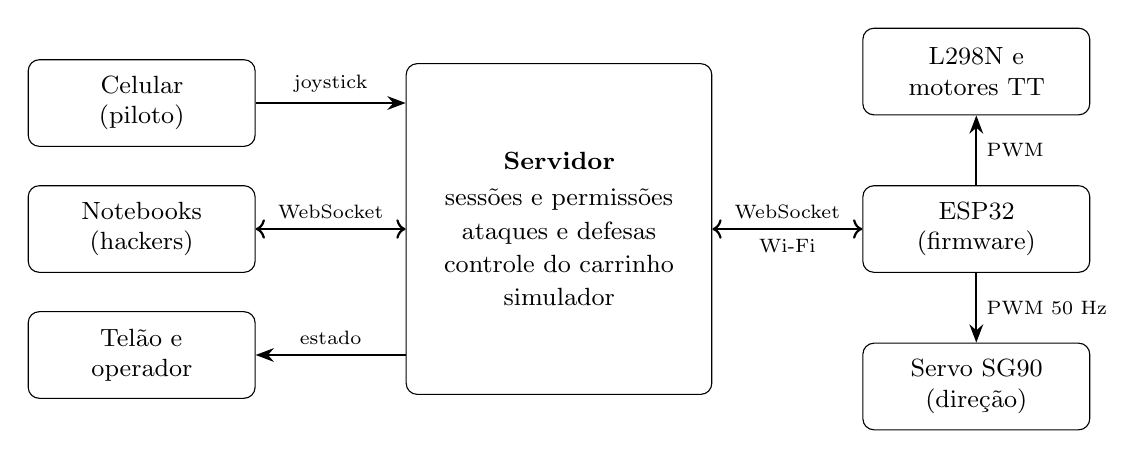
\begin{tikzpicture}[
  font=\small,
  caixa/.style={draw, rounded corners, align=center, minimum height=1.1cm, inner sep=4pt},
  seta/.style={-{Stealth}, thick}
]
\node[caixa, text width=2.6cm] (piloto) at (0,2.2) {Celular\\(piloto)};
\node[caixa, text width=2.6cm] (hacker) at (0,0.6) {Notebooks\\(hackers)};
\node[caixa, text width=2.6cm] (telao) at (0,-1.0) {Telão e\\operador};
\node[caixa, text width=3.6cm, minimum height=4.2cm] (srv) at (5.3,0.6) {\textbf{Servidor}\\[2pt]sessões e permissões\\[1pt]ataques e defesas\\[1pt]controle do carrinho\\[1pt]simulador};
\node[caixa, text width=2.6cm] (esp) at (10.6,0.6) {ESP32\\(firmware)};
\node[caixa, text width=2.6cm] (mot) at (10.6,2.6) {L298N e\\motores TT};
\node[caixa, text width=2.6cm] (servo) at (10.6,-1.4) {Servo SG90\\(direção)};
\draw[seta] (piloto) -- node[above, sloped, font=\scriptsize]{joystick} (srv.west |- piloto);
\draw[seta, <->] (hacker) -- node[above, font=\scriptsize]{WebSocket} (srv.west |- hacker);
\draw[seta] (srv.west |- telao) -- node[above, font=\scriptsize]{estado} (telao);
\draw[seta, <->] (srv) -- node[above, font=\scriptsize]{WebSocket} node[below, font=\scriptsize]{Wi-Fi} (esp);
\draw[seta] (esp) -- node[right, font=\scriptsize]{PWM} (mot);
\draw[seta] (esp) -- node[right, font=\scriptsize]{PWM 50 Hz} (servo);
\end{tikzpicture}
\fonte{Elaborado pelos autores (2026).}
\end{figure}

Os navegadores nunca falam direto com o carrinho. O comando do piloto vai ao servidor, passa pelos ataques e defesas ativos e só então segue para o ESP32. O servidor é a única autoridade sobre equipes, sessões, permissões e estado da partida; o que o navegador envia sobre papel ou equipe é ignorado, e essas informações vêm sempre da sessão.

\section{Componentes do carrinho}

A Tabela~\ref{tab:componentes} lista os componentes usados no carrinho e a função de cada um.

\begin{table}[htbp]
\centering
\small
\caption{Componentes do carrinho}
\label{tab:componentes}
\begin{tabularx}{\textwidth}{@{}P{5cm}L@{}}
\toprule
\textbf{Componente} & \textbf{Função} \\
\midrule
ESP32-WROOM-32 (placa de 38 pinos) & Microcontrolador com Wi-Fi e dois núcleos; recebe os comandos e aciona motores e servo. Fica numa placa de expansão com bornes de parafuso \\
Ponte H L298N & Driver dos dois motores: define o sentido de cada um e recebe o PWM de velocidade \\
2 motores TT amarelos com redução 1:48 (3 a 6~V) & Tração traseira, um motor por roda \\
Servo SG90 & Direção das rodas dianteiras \\
Regulador de tensão \emph{step-down} (LM2596, ajustado em 5~V) & Alimenta o ESP32 e o servo a partir da bateria \\
2 baterias 18650 em série & 7,4~V nominais (8,4~V carregadas), com chave liga e desliga \\
Peças impressas em 3D & Estrutura do carrinho \\
4 rodas de borracha de 64~mm & Rodas traseiras presas no eixo dos motores; dianteiras livres \\
\bottomrule
\end{tabularx}
\fonte{Elaborado pelos autores (2026).}
\end{table}

\section{Estrutura impressa em 3D}

A estrutura foi projetada em CAD e impressa em 3D. A base mede 200 por 140~mm e tem a frente estreitada para dar espaço às rodas esterçarem. Em cima ficam as bandejas do ESP32, da L298N e do regulador; embaixo ficam os suportes dos motores, o servo de cabeça para baixo e o mecanismo de direção (alavanca, barras e mangas de eixo). O carrinho tem cerca de 21 por 20~cm, entre-eixos de 98~mm e massa estimada de 630~g. É um carro para piso liso e interno.

O formato é o de um carro de verdade: tração nas rodas de trás e direção nas da frente. Ele não vira girando as rodas de um lado mais rápido que as do outro.

\section{Alimentação}

A bateria de 7,4~V alimenta dois ramos. O primeiro vai direto à L298N, que entrega a tensão aos motores. O segundo passa pelo regulador, que reduz para 5~V e alimenta o ESP32 e o servo. Todos os componentes compartilham o mesmo terra (GND). O servo nunca é ligado direto na bateria.

Como a L298N tem queda de cerca de 2~V e os motores são de até 6~V, o PWM dos motores foi limitado a 80\% no firmware. O servo e o ESP32 dividem o mesmo 5~V; para evitar que um pico de corrente reinicie o ESP32 (\emph{brownout}), o servo gira com velocidade limitada e os motores aceleram em rampa.

\section{Direção e tração}

\textbf{Direção}: o servo move uma alavanca ligada a duas barras de direção, numa geometria de Ackermann simplificada (na curva, a roda de dentro esterça mais que a de fora). O comando do piloto, de $-100\%$ a $+100\%$, é convertido em um ângulo de servo de até $\pm 45^\circ$, abaixo do batente mecânico de cerca de $48^\circ$. Todo comando passa por uma única função que aplica esse limite. No limite, o raio de curva previsto no CAD é de cerca de 27~cm. O servo gira no máximo a 250 graus por segundo.

\textbf{Tração}: cada motor é controlado por dois pinos de sentido e um pino de PWM na L298N, a cerca de 1~kHz. O piloto só escolhe frente, ré ou parar; a velocidade é fixa. Internamente o firmware usa uma rampa de aceleração de cerca de 150~ms e espera o motor parar antes de inverter o sentido. Para parar em emergência, o PWM dos dois motores vai a zero na hora, sem esperar a rampa.

\section{Firmware}

O firmware foi escrito em C++ com o \emph{framework} Arduino e o PlatformIO, e aproveita os dois núcleos do ESP32:

\begin{itemize}
  \item \textbf{Núcleo 0 -- tarefa de rede}: cuida do Wi-Fi, da conexão com o servidor, das mensagens e da telemetria.
  \item \textbf{Núcleo 1 -- laço de controle}: aplica os comandos ao servo e aos motores e verifica o tempo de validade de cada comando.
\end{itemize}

As duas partes trocam dados por filas. Assim, se a rede travar, o controle continua rodando e consegue parar o carrinho. Em teste com a rede presa por 3~s, o carrinho parou entre 347 e 399~ms.

Ao ligar, a primeira ação é deixar os motores desabilitados e o servo no centro. Só depois o firmware conecta à rede. A configuração é feita sem regravar o código: na primeira vez, o carrinho cria uma rede Wi-Fi própria; pelo celular, abre-se uma página onde se informam a rede do laboratório, o endereço do servidor, a identificação do carrinho e o segredo de autenticação, que ficam salvos na memória do ESP32.

\section{Sistema web}

O servidor roda no notebook, em TypeScript com Bun, Express e WebSocket. Ele concentra:

\begin{itemize}
  \item \textbf{Sessões e permissões}: login com senha guardada como \emph{hash} argon2id, uma vaga por papel e verificação da permissão a cada mensagem.
  \item \textbf{Máquina de estados da partida}: configuração, pronto, em andamento, pausado e encerrado. Ao sair de \enquote{em andamento}, todos os carros param.
  \item \textbf{Cadeia de comandos}: o comando do piloto passa pelos ataques ativos (replay, travamento, viés e inversões) e pelas defesas, que podem bloquear as alterações. O comando de parada nunca passa pelos ataques.
  \item \textbf{Controle do carrinho}: numera os comandos, limita o envio a 20 por segundo, dá prioridade à parada e para o carro se o piloto deixar de mandar comandos.
  \item \textbf{Simulador}: um carrinho virtual com a mesma lógica do firmware, que permite jogar sem hardware e serve de plano B na apresentação.
\end{itemize}

As interfaces foram feitas em React com TypeScript. Há telas para o piloto (joystick para toque e teclado), para os hackers (abas de ataque e defesa), para o operador (controle da partida, código QR para os celulares entrarem e métricas) e para o telão. Todas as mensagens entre navegador e servidor são validadas por esquemas compartilhados (Zod); mensagens fora do formato são recusadas.

\section{Comunicação entre o ESP32 e o servidor}

O notebook, os celulares e o ESP32 ficam na mesma rede Wi-Fi de 2,4~GHz. O ESP32 mantém uma conexão WebSocket com o servidor, por onde trafegam mensagens em JSON de até 512 bytes. A Tabela~\ref{tab:mensagens} resume as mensagens.

\begin{enumerate}
  \item \textbf{Conexão e autenticação}: o ESP32 abre a conexão e, em até 3~s, envia sua identificação e um segredo. Se estiverem corretos, o servidor responde com as boas-vindas e o tempo de validade dos comandos; se não, fecha a conexão. Se o mesmo carrinho conectar de novo, a conexão antiga é substituída.
  \item \textbf{Comando}: cada comando de movimento leva um número de sequência, a tração (ré, neutro ou frente), a direção ($-100$ a $+100$) e um tempo de validade de 400~ms. O firmware só aceita números de sequência maiores que o último recebido e valores dentro da faixa; caso contrário, recusa e para.
  \item \textbf{Confirmação}: depois de aplicar um comando, o ESP32 responde com os valores que realmente aplicou. É isso que o telão mostra como \enquote{confirmado}, ao lado do \enquote{solicitado} pelo piloto.
  \item \textbf{Telemetria}: a cada 500~ms o ESP32 envia tempo ligado, intensidade do sinal Wi-Fi, último comando, posição atual e contadores de falhas. O servidor manda um sinal de vida a cada 1~s.
  \item \textbf{Parada}: um comando de parada é sempre obedecido, mesmo fora de ordem. Quando o carrinho para por conta própria, ele informa o motivo.
\end{enumerate}

\begin{table}[htbp]
\centering
\small
\caption{Mensagens entre servidor e ESP32}
\label{tab:mensagens}
\begin{tabularx}{\textwidth}{@{}P{3.4cm}P{3.6cm}L@{}}
\toprule
\textbf{Mensagem} & \textbf{Sentido} & \textbf{Conteúdo} \\
\midrule
\texttt{device.hello} & ESP32 $\rightarrow$ servidor & Identificação do carrinho, segredo e versão do firmware \\
\texttt{device.welcome} & servidor $\rightarrow$ ESP32 & Confirma a autenticação e informa a validade dos comandos \\
\texttt{device.drive} & servidor $\rightarrow$ ESP32 & Sequência, tração, direção e validade \\
\texttt{device.stop} & servidor $\rightarrow$ ESP32 & Parada imediata, com o motivo \\
\texttt{device.heartbeat} & servidor $\rightarrow$ ESP32 & Sinal de vida; não mantém o carro andando \\
\texttt{device.ack} & ESP32 $\rightarrow$ servidor & Valores aplicados de fato \\
\texttt{device.telemetry} & ESP32 $\rightarrow$ servidor & Estado do carrinho a cada 500~ms \\
\texttt{device.stopped} & ESP32 $\rightarrow$ servidor & Aviso de parada e motivo \\
\texttt{device.fault} & ESP32 $\rightarrow$ servidor & Mensagem inválida recebida \\
\bottomrule
\end{tabularx}
\fonte{Elaborado pelos autores (2026).}
\end{table}

\subsection{Parada segura}

A regra mais importante do sistema é que o carrinho pare sozinho quando algo dá errado. Enquanto o piloto segura o joystick, o celular reenvia o comando a cada 100~ms. Cada comando vale por 400~ms. Se o piloto soltar o joystick, se a rede cair ou se um ataque atrasar ou bloquear os comandos, o comando expira e os motores desligam. Essa verificação existe em duas camadas, no servidor e no firmware, e nenhum ataque consegue desligá-la. O sinal de vida do servidor não renova a validade, então uma conexão aberta sem comandos não mantém o carro andando.

O firmware também vigia o silêncio da rede: depois de 1,5~s sem nenhuma mensagem do servidor, para de enviar telemetria; depois de 5~s, fecha a conexão e reconecta. Ao reconectar, o carrinho continua parado até receber um comando novo do piloto.

\subsection{Onde os ataques acontecem}

Todos os ataques são aplicados dentro do servidor, entre o piloto e o carrinho. Para o firmware, um ataque aparece apenas como um comando com valores alterados, um intervalo maior entre comandos ou uma parada. Por isso o ESP32 não precisou mudar para receber os novos ataques, e a parada segura continua valendo durante todos eles.

\section{O que é real e o que é simulado}

São proteções reais: autenticação por senha com \emph{hash} argon2id e política de senha forte; desconexão do piloto quando a senha muda; sessões em \emph{cookie} protegido; autorização a cada mensagem; limite de tentativas contra força bruta; verificação de origem das conexões; autenticação do ESP32 por segredo; e a parada segura em duas camadas.

São simulações didáticas: as etapas de invasão, a integridade (não é uma assinatura criptográfica como HMAC), a proteção contra repetição e a criptografia (não é TLS; a rede trafega em texto claro). Essa separação é explicada ao público, para não passar a ideia de que o sistema é seguro só porque o indicador está cheio.

\chapter{Resultados e validação}

\begin{itemize}
  \item \textbf{Software}: \emph{lint}, verificação de tipos, \emph{build} e 343 testes automatizados aprovados. Os testes de ponta a ponta direcionados aos ataques novos e aos textos educativos passaram (16 de 16, em desktop e celular emulado). A suíte completa de ponta a ponta não foi concluída após os últimos ajustes.
  \item \textbf{ESP32 real com saídas desligadas}: 23 de 23 verificações dos ataques pelo protocolo real. O firmware confirmou inversão, viés, travamento, replay e sequestro; a perda de 60\% dos pacotes acionou a parada automática.
  \item \textbf{Bancada com motores e servo soltos}: 18 de 18 verificações, com observação física parcial, e uma partida de ataque e defesa.
  \item \textbf{Parada segura}: com a rede travada por 3~s, o carrinho parou logicamente entre 347 e 399~ms.
  \item \textbf{Rede}: o \emph{hotspot} do celular em 2,4~GHz ficou 30 minutos sem queda; a rede \emph{mesh} doméstica caía a cada cerca de 5 minutos e foi descartada.
\end{itemize}

\section{Limitações}

O carrinho ainda não foi testado montado no chassi nem andando no chão; os testes físicos foram feitos com motores e servo soltos. A alimentação do ESP32 apresentou queda de cerca de 0,5~V por contatos de protoboard e será refeita. A rede é aberta (sem TLS), aceitável apenas no laboratório isolado.

\chapter{Conclusão}

O HIJACK cumpre o objetivo de tornar visível algo que normalmente é invisível. Quando o carrinho vira para o lado errado ou é sequestrado porque a senha era \texttt{1234}, o público entende na prática o que aconteceu com os refrigeradores na Europa; quando o carrinho para sozinho porque a rede caiu, entende por que sistemas críticos precisam de um modo seguro de operação quando a rede falha, como o Porto de Santos, que manteve navios e acessos funcionando por meios alternativos.

Os casos de 2025 e 2026 mostram que a IA acelerou os dois lados: ela orquestrou invasões (GTG-1002), ajudou a achar falhas antigas em poucos dias (PHP2Shell) e foi usada para avançar dentro de uma empresa (Binance), mas também foi usada para construir este projeto. As defesas básicas continuam decisivas: trocar senhas padrão, atualizar sistemas rapidamente, verificar a integridade do que se instala e projetar equipamentos para falhar de forma segura.

Como próximos passos ficam a montagem no chassi, os testes no chão e no local da apresentação, e a avaliação de novas defesas.

\postextual

\bibliography{referencias}

\end{document}
